\documentclass[11pt, oneside]{article}      % use "amsart" instead of "article" for AMSLaTeX format
\usepackage[top=1.25in, bottom=1.25in, left=1in, right=1in]{geometry}                       % See geometry.pdf to learn the layout options. There are lots.
\geometry{letterpaper}                          % ... or a4paper or a5paper or ... 
%\geometry{landscape}                       % Activate for for rotated page geometry
\usepackage[parfill]{parskip}           % Activate to begin paragraphs with an empty line rather than an indent
\usepackage{graphicx}               % Use pdf, png, jpg, or eps§ with pdflatex; use eps in DVI mode
                                % TeX will automatically convert eps --> pdf in pdflatex        
                                
\usepackage[justification=centering]{caption}                               
\usepackage[justification=centering]{subcaption}             
\usepackage{amssymb}
\usepackage{amsmath}

\newcommand{\word}{\textnormal{word}}
\newcommand{\lemma}{\textnormal{lemma}}

\title{Machine Translation \\ Final Project Report}
\author{Jeremy Silver}
\date{Thurs.\ 5/7/15}                          % Activate to display a given date or no date

\begin{document}
\maketitle

\section{Introduction}

For my final project, I have developed a miniature MT system that I dub ``HOLI QUAIL'' (Higher-Order Logic Interpreted Quantificational Interlingua).  As the name suggests, it uses an interlingua-based approach to machine translation, where it first interprets a sentence in the source language into \textbf{higher-order logic} (HOL), which is an extension of first-order logic that allows for quantification over predicates.  The logic is equipped with a language-neutral lexicon of terms that can be logically combined.  From the interlingua representation, sentences can then be generated in the target language.  Throughout the process, syntactic transformations are executed in accordance with the \textbf{X-bar theory} of Chomskyan linguistics.  

At present, HOLI QUAIL is capable of translating simple sentences of Japanese into English, but the methodology is easily generalized to other languages.  In the first half of this paper, we will give a broad survey of interlingua methods, as well as the syntactic and semantic theories underlying HOLI QUAIL.  In the second half, we delve into the implementation specifics.

\section{A Brief Review of Interlingua-Based Machine Translation and Reasoning }

The notion of translating various tongues into a common intermediary is hardly new, and it can be said to go back at least as early as Leibniz in the 18th century with his \textit{characteristica universalis}.  There was a great deal of emphasis in the 1950s and '60s on the formal representation of language as the computer age was dawning, and as Noam Chomsky was beginning to expound the basis of his theories of generative grammar.  

Some early efforts that created a lot of enthusiasm towards automated language understanding were \textbf{ELIZA} and \textbf{SHRDLU}, computer programs written at MIT in the 1960s.  ELIZA is a chat robot designed to emulate a psychotherapist, issuing evasive responses like ``Can you elaborate on that?'' whenever it was incapable of grasping the human's statement.  As basic as ELIZA's methods were, it was still able to convince quite a few people that it was really human.

Then there was SHRDLU, which allowed a user to interact with the computer by making queries about a fictitious universe containing ``blocks'' of various shapes and sizes.  The program was built with an \textbf{ontology}, a set of objects and relations with which it could reason.  This is an interlingua in the sense of being a well-defined formal representation of the world, and the domain-specific natural language queries made by the human could be translated into SHRDLU's formal language of blocks and relations.  The project succeeded as a proof-of-concept, but it failed to scale up to larger domains of natural language that feature a lot of ambiguity and complex reasoning.  

Many attempts have been made since SHRDLU to get computers to understand language, but most have met with a similar fate as they attempted to climb the mountain of complexity.  Efforts continued for the next few decades, which were aided by the evolving linguistic theory.  Some modern incarnations of interlingua-based MT are \textbf{UNITRAN} and \textbf{KANT}, which were developed in the 1990s.  MIT's UNITRAN uses Government \& Binding Theory (a predecessor to X-bar theory) as its syntactic system, and it interprets sentences into a Lexical Conceptual Structure encoding the semantic relationships conveyed in the sentence.  This interlingual representation is then used to \textit{generate} sentences in the target language.  Carnegie Mellon University's KANT is similar in its workflow (see Figure \ref{kant_workflow}), but it also brands itself as a ``knowledge-based'' system that uses statistical corpus-mining to acquire a semantic and pragmatic knowledge base, thus improving its flexibility in handling ambiguity and uncertainty.  

\begin{figure}[h]
\centerline{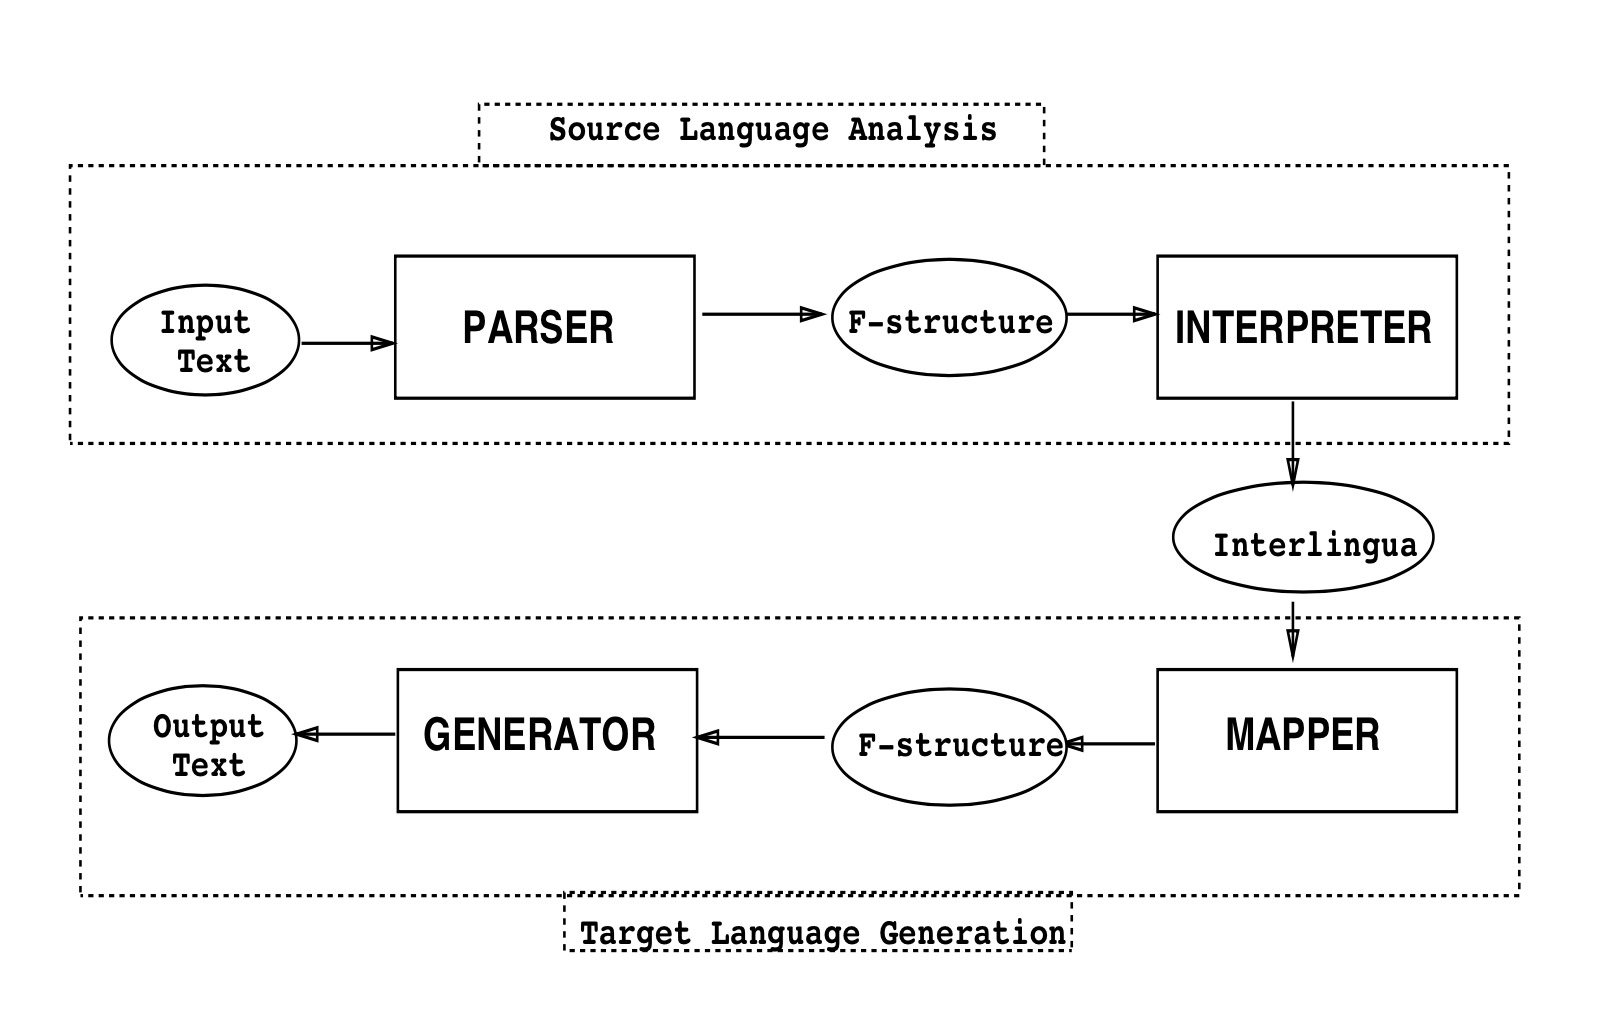
\includegraphics[scale=1]{kant.jpg}}
\caption{Four modules of the KANT MT system} \label{kant_workflow}
\end{figure}

Unfortunately, although these projects held promise and were beginning to reach the point of deployability, they seem to have fallen by the wayside as the computation boom allowed statistical methods to rise to prominence in the last two decades.  In light of these advances and the recent successes of sophisticated AI systems such as IBM Watson, the way forward seems to be a hybrid approach involving formal linguistic theory, abstract representations, and statistics.

\section{Why Interlingua?}

As indicated, interlingua MT efforts have waned in recent times due to the contrastively high growth rate of statistical MT, and due to the immense difficulties involved in: (a) establishing an agreed-upon set of primitives for the ontology and grammar, and (b) scaling a system up from SHRDLU's self-contained ``block world'' to the vast (and exceedingly messy) domain of ``all languages.''  Still, from a theoretical point of view, interlingua-based MT has several advantages.  First, the interlingua allows the translation to occur in two steps, and it keeps the source language independent of the target language.  This means that one only needs to consider translation between each language and the interlingua, instead of between each pair of languages.  The number of systems that need to be built is now $O(N)$ in the number of languages, rather than $O(N^2)$.

Also, many of the techniques abstract away from the lexical level and even from the language level, meaning that the same set of rules can apply universally to all languages.  In this sense it is highly modular, and the user only needs to ``plug in'' a lexicon and a small set of parameters specific to the language.

A final motivation for rule-based methods is that they are expert-driven.  While processing large corpora can certainly be helpful for solving certain problems (discussed further in Section \ref{stats}), it may be relatively ineffective at teasing out the deeper structure of language.  The large amount of data may be superfluous anyway if the language can be encoded in a handful of simple rules.  Instead of spending many hours on intensive training algorithms, the syntactic model and the lexicon will be designed from the start to incorporate the nuanced insights of language experts.  

\section{Theoretical Preliminaries}

Before describing the implementation details of HOLI QUAIL, we now present the reader with some linguistic background on how we plan to represent each level of structure.

\subsection{Syntax: X-bar theory}

To spare the reader a lengthy discourse on X-bar theory, here is a list of some central principles:

\begin{enumerate}
\item Every meaningful phrase is the root of some tree structure, called a \textbf{constituent}.  Furthermore, trees are always at most binary-branching.  One child of every node is considered the \textbf{head}, which confers its part of speech and other morphological features to its parent node.
\item Lexical and morphological features interact with the syntax to constrain the set of possible trees.
\item Language is recursive; that is, a constituent can be comprised of subconstituents, with no upper bound to the amount of regress.  Furthermore, constituents of the same category are intersubstitutable.  
\item Sentences have a \textbf{deep structure}, or underlying form, that is closely related to their logical form.  Movement operations are then applied to the syntax tree to satisfy the constraints of the grammar.
\item All languages have commonalities in terms of the basic rules of syntax, but they may have different \textbf{parameters} determining which structures are well-formed.  For example, in English, every sentence must have an explicit subject, but in Japanese and many other languages, subjects are optional.
\end{enumerate}

Much of syntactic theory is devoted to explaining complex movement operations on syntax trees that can account for linguistic observations.  One important concept is that of a \textbf{trace}, which is left behind when a syntactic constituent moves to some other position in the tree.  For example, in \textit{wh}-movement, a question phrase beginning with \textit{wh} moves to the beginning of the sentence.  So in the sentence, ``Which movie did you see?", the deep structure is ``You saw which movie?" and that ``which movie" moves to the front.  However, this would separate the transitive verb ``saw'' from its direct object, and it would no longer be a constituent.  To solve this problem, the hypothesis is that ``which movie'' leaves behind a trace: ``Which movie$_1$ did you see \textit{t}$_1$?"  This trace, $t_1$, can be interpreted as a bound variable that is co-indexed to the phrase ``which movie.''  Awareness of these traces will be crucial when we discuss quantifier movement in Section \ref{quantification}.

X-bar theory also asserts that phrases represent a \textbf{maximal projection} of the lexical category, and that intermediate projections  (X$'$) come between the lexical entry itself (X) and the final phrase (XP) that it heads.  For example, observe how in Figure \ref{john_runs} the X-bar sentence structure of ``John runs" is relatively complicated despite the simplicity of the sentence.  The categories that can stand in for X include N (noun), D (determiner), Adj (adjective), V (verb), T (tense), and P (preposition).  The difference between a VP and a TP is that a TP includes all the information about the verb's tense, mood, and aspect.  In the example sentence, the verb phrase rises to a $T'$ even without an overt T word.  (In fact, the T is embodied in the plural marker `s' that comes at the end of `runs').

\begin{figure}[h] 
\centerline{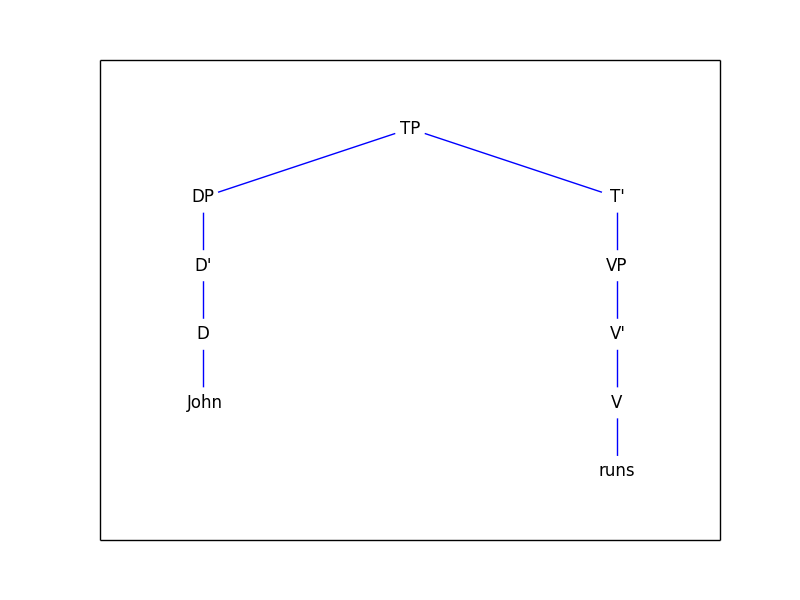
\includegraphics[scale=.6]{runs_eng_1.png}}
\caption{X-bar theory and projection} \label{john_runs}
\end{figure}

\subsection{Semantics: Compositionality and HOL} \label{compositionality}

Unique to each language is its lexicon, which in its basic sense is a mapping from words to meanings.  Unfortunately, ``meaning'' is an extremely vague term that the author has no intention of elucidating.  However, given a set of \textbf{atomic concepts} that we take as given, our goal is to assign to each word a higher-order logical expression combining these concepts.  We use the formalism of a \textbf{typed lambda calculus} to achieve this.  

In typed higher-order logic, every expression must be assigned a type, and every type is either a basic type or the signature of a function from one type to another.  That is, $e$ and $t$ are the basic types, and if $\sigma$ and $\tau$ are types, then ${<}\sigma, \tau{>}$ is the type of functions from $D_{\sigma}$ to $D_{\tau}$, where $D_{\sigma}$ and $D_{\tau}$ are the domains of objects with types $\sigma$ and $\tau$ respectively.  $D_e$ is the set of primitive ``entities,'' or ``things in the universe,'' while $D_t = \{0, 1\}$ is the set of truth values.  Sentences have $t$ as their semantic type, individuals have $e$ as their type, and unary predicates (like intransitive verbs) have ${<}e, t{>}$ as their type.  Here are some examples of lexical entries with their corresponding logical expressions (called \textbf{denotations}) and types:

\begin{itemize}
\item ``John'' $\; \rightarrow \;$ JOHN, \quad \quad \quad type: $e$
\item ``runs'' $\; \rightarrow \;$ $\lambda x \, . \, $RUN$(x)$, \; type: ${<}e, t{>}$
\end{itemize}

The $\lambda x$ in the previous expression is a convenient shorthand notation for ``function that maps $x$ to RUN$(x)$.'' In general, whatever comes after the $\lambda$ but before the period is a listing of argument variables, and whatever comes after the period is the function output, which is allowed to include the argument variables.  The reader may wonder what is accomplished by defining our terms by simply capitalizing them, but actually this is just a convenient way of designating that these are among our ``atomic concepts.'' 

Semantics interacts with syntax via the \textbf{principle of compositionality}:\ the denotation of a parent node is determined solely by the denotations of its child nodes.  The primary rule by which they combine is \textbf{function application}; when two constituents of a syntax tree are sisters, the denotation of the parent is the result of applying the denotation of one sister (as a function) to the other.  Which constituent is the function and which is the argument can always be determined by the type signature. Hence in our example, by function application, the denotation of ``John runs'' is the function RUN applied to the argument JOHN, with a return value of type $t$.  (In fact, all sentences have type $t$).

A natural objection to raise at this point is that, if the sentence has the structure shown in Figure \ref{john_runs}, then ``John'' and ``runs'' are not sisters.  This requires the addition of another rule, that of \textbf{vacuous projection}: if node $a$ has node $b$ as its only child, then the denotation of $a$ is the same as the denotation of $b$.  In this way, the denotation of ``John'' gets projected up to its DP ancestor, and the denotation of ``runs'' gets projected up to its T$'$ ancestor, at which point the denotations are allowed to combine by function application.

Another rule we will need is that of \textbf{predicate modification}.  If the type of common nouns is ${<}e, t{>}$, then function application will not apply if we try to combine an adjective with a noun.  Instead we need to take the intersection of the two predicates.  For example, the noun phrase ``happy donkey'' will be the intersection of $\lambda x \, . \, $HAPPY$(x)$ and $\lambda x \, . \, $DONKEY$(x)$, which is $\lambda x \, . \, $HAPPY$(x) \, \wedge \, $DONKEY$(x)$.

\subsection{Quantification} \label{quantification}

We need one more rule in order to semantically interpret simple sentences in HOL, but this one will be much more of a challenge.  The issue is that of \textbf{quantificational expressions}, such as ``a chair'', ``every farmer'', or ``no donkey.''  We run into a problem when we try to combine these phrases with predicates as we did with ``John runs.''  For example, take the sentence ``No donkey is happy.'' By the type signatures we have used so far, the expression ``is happy'' (with a vacuous verb ``is'') should have predicate type ${<}e, t{>}$.  If ``every donkey'' has type $e$, as ``John'' did, then how do we assign a denotation of that type to it?  Items of type $e$ are supposed to be individuals, and ``no donkey'' is clearly not an individual.  The only solution seems to be to change the type of quantificational DPs like ``no donkey'' to ${<}{<}e, t{>}, t{>}$ so that they can instead take the \textit{predicate} as an argument.  This makes good sense, since the phrase ``no donkey'' can readily be given the denotation $\lambda P \, . \, \neg \exists x \, . \, $DONKEY$(x) \, \wedge \, P(x)$.  This is the characteristic function of predicates that are not satisfied by any donkey.  This discovery leads to the interpretation of the bare determiner ``no'' to be $\lambda Q \, . \, \lambda P \, . \, Q(x) \, \wedge \, P(x)$.  

This leads us to another problem, that of quantificational DPs in object position.  For example, in ``Every farmer has a donkey," the constituent ``has a donkey'' would have to have type $t$ by our previous analysis, as opposed to the ${<}e, t{>}$ that we desire.  There are two mechanisms we will use to handle this.  The first is a syntactic operation called \textbf{quantifier raising}, which moves the quantified DP to the beginning of the sentence, and leaves behind a trace of type $e$ in its place, whose index is bound to the DP.  The second is \textbf{predicate abstraction}, which is a semantic operation that allows us to take a term of type $t$ with a free variable, and turn it into a predicate, which is just a lambda function that binds the free variable.  The trace of type $e$ allows us to use function application to assign the denotation HAS$(x)$ to the combination of ``has'' with the trace.  Then, after predicate abstraction, we bind the free variable to get $\lambda y \, . \, $HAS$(x)$, which has a valid predicate type that can combine with ``every farmer.''  Finally, the QR'ed DP ``a donkey'' takes the abstracted predicate $\lambda y \, . \, \forall x \, . \, $FARMER$(x) \, \rightarrow \; $HAS$(y, x)$ as an argument, in order to produce the final expression:
$$
\exists y \, . \, \textnormal{DONKEY}(y) \, \wedge \, \forall x \, . \, \textnormal{FARMER}(x) \, \rightarrow \, \textnormal{HAS}(y, x).
$$

However, if we stop here, we are forced to accept the above expression as the denotation of the sentence.  This is called the \textbf{wide scope} reading, since the scope of the inner phrase ``a donkey'' has moved to encompass the outer phrase ``every farmer.''  This is not the most natural reading, though, so in order to generate the more natural \textbf{narrow scope} reading, $\forall x \, . \, $FARMER$(x) \, \rightarrow \, \exists y \, . \, $DONKEY$(y) \, \wedge \, $HAS$(y, x)$, we need to apply QR and predicate abstraction to the subject DP as well, and these must apply \textit{after} the object DP is moved in order to get wider scope.  This turns out to be a very nice solution (albeit somewhat complicated), because it accounts for the two alternative readings of the sentence.

A final note: for the sake of uniformity, it makes sense to assign proper nouns the category D instead of N, so that they can project up to full DPs on their own and be given the type ${<}{<}e, t{>}, t{>}$.  The denotation of ``John'', then, is no longer simply JOHN, but rather $\lambda P \, . \, P($JOHN$)$.  Conceptually, this can be thought of as ``the set of properties true of John.''

\begin{figure} [ht]
\centerline{
\begin{minipage}[c]{0.5\linewidth}
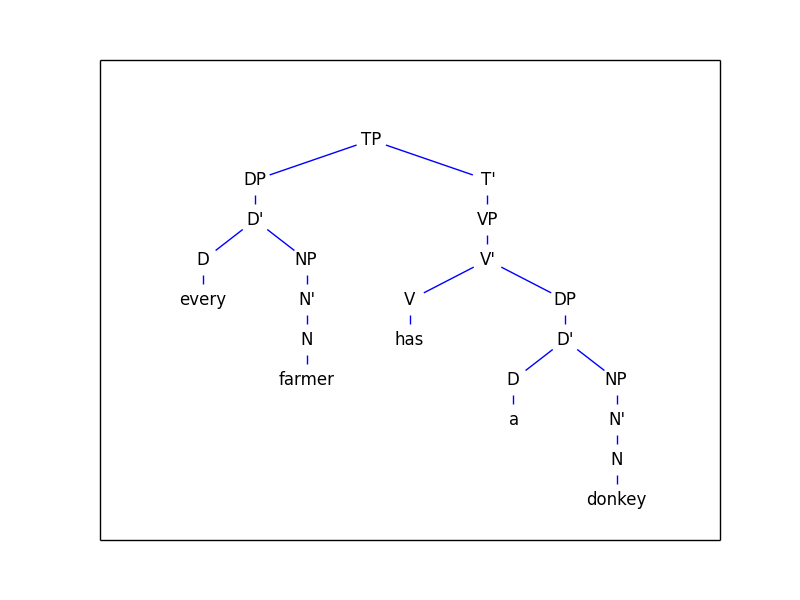
\includegraphics[scale=.5]{donkey_eng_1.png} 
\subcaption{}
\end{minipage}} 
\begin{minipage}[c]{0.5\linewidth}
\centering
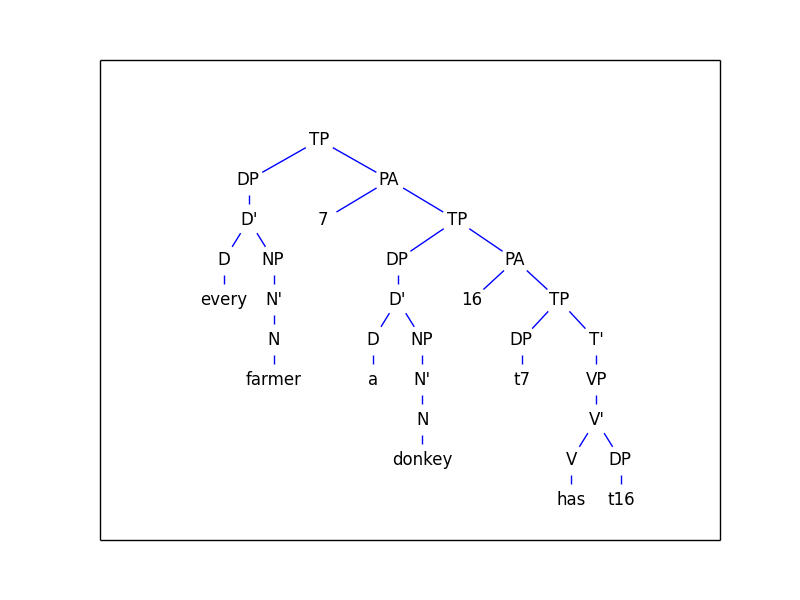
\includegraphics[scale=.43]{donkey_eng_2.png}
\subcaption{}
\end{minipage}
\begin{minipage}[c]{0.5\linewidth}
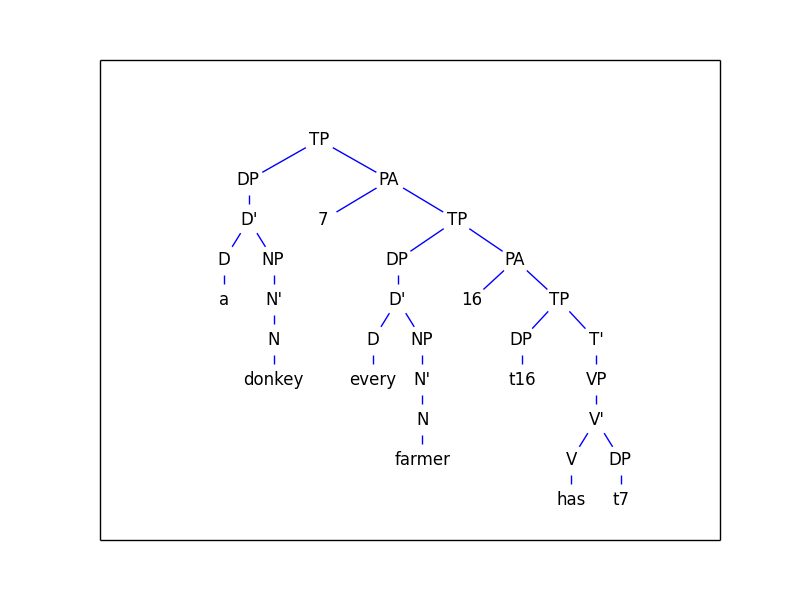
\includegraphics[scale=.43]{donkey_eng_2_2.png}
\subcaption{}
\end{minipage}
\caption{Quantifier Raising and Predicate Abstraction \\ (a) Surface structure, (b) Narrow scope, (c) Wide scope} \label{QR}
\end{figure}

\section{HOLI QUAIL: An Overview}

With the technical machinery in hand, we can now describe the implementation of HOLI QUAIL.  This translation system uses \textbf{logical equivalence} as its standard for translation, in that it attempts to generate every possible sentence it can in the target language that is logically equivalent to the source sentence.  This is a strong condition, but it is useful because it is abstract enough to capture major differences in syntax between languages.  Another unique feature of the system is that it can handle the quantificational scope issues discussed in the previous section.

HOLI QUAIL processes a sentence in phases nearly identical to those shown in Figure \ref{kant_workflow}.  It starts by parsing the sentence into X-bar theory, then interprets it using the rules of compositional semantics.  Next, it generates semantically equivalent syntax trees in the target language, using HOL as the interlingua.  Finally, it applies lexical lookups and syntactic/morphological transformations to recover a well-formed sentence in the target language.  

It is important to keep in mind that \textbf{ambiguities} can crop up in almost every stage of the process, and as we proceed through each step in the next few sections, we will describe the kinds of ambiguities that can occur.  In our system, we do not resolve ambiguities by choosing among them, but instead we attempt to deterministically produce all possible outputs.  Python has an extremely handy data type called a \textbf{generator}, which is a means of lazily generating the next output whenever \texttt{next()} is called, so that even if there is a large number of possible outputs, we can generate only the first few of them if we so choose. 

We refer the reader to the source code, found in the main \texttt{project} directory, in order to follow along.  Most of the algorithm is in \texttt{sem.py}, with other auxiliary components in other files.

\subsection{Input sentence to surface structure tree}

First we create a \textbf{context-free grammar} that encodes the rules of X-bar theory specific to a particular language.  (See \texttt{english.fcfg} and \texttt{japanese.fcfg}).  This specifies both the lexical production rules, which identify which categories and \textbf{morphological features} pertain to each word, as well as the higher-level production rules, such as
\begin{verbatim}
TP[TENSE=?t, NUM=?n, PERSON=?p] -> 
    DP[NUM=?n, PERSON=?p] TBar[TENSE=?t, NUM=?n, PERSON=?p]}
\end{verbatim}
The items in brackets specify indicate that the morphological features are tied together in a certain way.  For instance, the tense of the parent TP node must match the tense of its T$'$ child, and the person and number of all three nodes must be in agreement.  This feature-matching constraint represents \textbf{subject-verb agreement} in this example.

Once we have the CFG file, we can use NLTK's\footnote{Python's Natural Language Toolkit.} \texttt{parser} module to parse an input sentence according to these rules.  The \texttt{parse} method returns a generator of syntax trees, which will be empty if there are no valid parses, and will contain more than one tree if there is syntactic ambiguity.  An example of such ambiguity is, ``I saw the man with the telescope."  (Note: at present, \texttt{english.fcfg} is not yet capable of handling prepositional phrases, so opportunities for syntactic ambiguity are scarce so far).

\subsection{Surface structure tree to deep structure tree}

For each surface structure tree, we then apply syntactic movement operations to obtain the deep structure that is capable of generating a logical form.  There are all sorts of movement possible, such as the \textit{wh}-movement described earlier, but for now we have only implemented quantifier raising, since it is the most important for handling basic quantification (and in our model, all DPs are quantified, even proper nouns).

Because multiple DPs may be raised, this induces a potential number of scope ambiguities equal to $n!$, where $n$ is the number of DPs.  The ordering of proper nouns does not affect the logical form, though, since there is no interchange of quantifier ordering.  Also, a pair of existential quantifiers or a pair of universal quantifiers will generate equivalent logical expressions regardless of their order, so in practice scope ambiguities are rare.

There are some significant complications when translating Japanese, though.  In particular, the language does not have obligatory determiners the way English does, so it lacks the definite and indefinite articles ``the'' and ``a.''  Consequently, either alternative might be possible, so HOLI QUAIL generates both possibilities whenever a determiner is absent.  Also, due to the topicalized structure of a Japanese sentence, we do not allow objects to have wider scope than subjects.

\subsection{Deep structure tree to HOL}

The next phase is a straightforward application of the four compositionality rules described in Sections \ref{compositionality} and \ref{quantification}.  Starting from each leaf (i.e.\ word) of the tree, we look up the lexical entry in the lexicon (see \texttt{lexicon.py}).  Its semantic type must correspond to its grammatical category (its parent in the tree), and there may be lexical ambiguity that arises from polysemy (think ``glasses'' meaning either spectacles or drinking cups), though at present we do not include any polysemous entries.

Other than multiple lexical entries, there should be no other kinds of ambiguity that arise here.  But if a composition failure occurs at any point, the null generator is returned.  If the semantic interpretation manages to proceed successfully all the way to the root of the tree, then the sentence has been successfully assigned a denotation in higher-order logic.  This is the interlingual representation of the sentence, which in theory can be used to generate sentences in any target language provided the lexicon and grammar are specified.

\subsection{HOL to Natural Language Logic}

We now begin the process of mapping the interlingua to the target language, and the next step is probably the most challenging.  The logic expression itself has a structure to it, but it does not necessarily correspond to the syntax of the target language.  Most languages, like English, tend to attach quantifiers to predicates that restrict the domain of the quantified variable.  ``Every farmer'', for instance, basically applies a universal quantifier to the predicate that follows it, but it also restricts the domain of the quantified variable to the set of farmers.  So in the sentence ``Every farmer is happy", we say that the predicate FARMER is the \textbf{restrictor} and the predicate HAPPY is the \textbf{nucleus}.  Our interlingua will give this sentence the denotation
$$
\forall x \; . \; \textnormal{FARMER}(x) \, \rightarrow \, HAPPY(x).
$$
It is fairly straightforward to convert this formula into a slightly different logical language, which we dub \textbf{Natural Language Logic} (NLL):
$$
\textnormal{EVERY} \; x \; | \; FARMER(x) \; . \; HAPPY(x).
$$
One can read this as, ``for every $x$ such that $x$ is a farmer, $x$ is happy.''  In this way, we have separated the quantified predicate into its restrictor and nucleus components.  

Things become more difficult when we consider existential quantification.  Consider now the sentence ``A farmer is happy.''  Its HOL denotation is
$$
\exists x \; . \; \textnormal{FARMER}(x) \, \wedge \, \textnormal{HAPPY}(x).
$$
Due to the symmetry of the conjunction expression (as opposed to the asymmetric implication given by ``every''), it is now unclear how to split the predicate into restrictor and nucleus.  In fact, there are six possibilities:
\begin{enumerate}
\item $\textnormal{SOME} \; x \; | \; \textnormal{FARMER}(x) \; . \; \textnormal{HAPPY}(x) \quad \quad \quad \; \; \Rightarrow \quad \textnormal{``A farmer is happy."}$ 
\item $\textnormal{SOME} \; x \; | \; \textnormal{HAPPY}(x) \; . \; \textnormal{FARMER}(x) \quad \quad \quad \; \; \Rightarrow \quad \textnormal{``Some happy thing is a farmer."}$
\item $\textnormal{SOME} \; x \; | \; \textnormal{HAPPY}(x) \, \wedge \, \textnormal{FARMER}(x) \; . \; ( \; ) \quad \Rightarrow \quad \textnormal{``A happy farmer exists."}$
\item $\textnormal{SOME} \; x \; | \; \textnormal{FARMER}(x) \, \wedge \, \textnormal{HAPPY}(x) \; . \; ( \; ) \quad \Rightarrow \quad \textnormal{``A farmer who is happy exists."}$
\item $\textnormal{SOME} \; x \; | \; ( \; ) \; . \; \textnormal{HAPPY}(x) \, \wedge \, \textnormal{FARMER}(x) \quad \Rightarrow \quad \textnormal{``There is a happy farmer."}$
\item $\textnormal{SOME} \; x \; | \; ( \; ) \; . \; \textnormal{FARMER}(x) \, \wedge \, \textnormal{HAPPY}(x) \quad \Rightarrow \quad \textnormal{``There is a farmer who is happy."}$
\end{enumerate}
All of these expressions are (arguably) logically equivalent, meaning they are all valid translations.  Unfortunately, the number of possibilities will combinatorially explode as the number of conjuncts increases (the exact number should be $(k + 1) k!$, where $k$ is the number of conjuncts).

However, we note that some of these translations sound much more natural than others (\#2, for example, is so awkward as to be easily ruled out, even though it is grammatical).  That is, the target language has a preferred order of modifying words.  Another example of this is how in English we typically put colors right before the noun, thus preferring ``big red ball'' to ``red big ball.''  Using heuristics such as these, we can generate outputs in some kind of plausibility order, or rule out certain orderings entirely.  

\subsection{Natural Language Logic to deep structure tree}

The next phase involves converting an NLL expression into a syntax tree.  This process is deterministic and ambiguity-free.  First, each quantifier and restrictor clause is stripped away from the NLL expression and converted into a quantified DP in the syntax tree in pre-sentence QR position.  Then the ``semantic core'' is converted into the remainder of the tree (a TP) using the specific syntactic rules of the target language.  For the moment, we ignore morphology and allow the lexical terminals to be ``morphology-bare'' terms.  For example, the semantic core HAPPY$(x)$ would generate a TP tree with a trace in subject position, the morphology-bare verb BE as the terminal verb, and HAPPY as the terminal adjective.  Afterwards, the inverse of QR takes place, and quantified DPs are lowered back into the positions occupied by their corresponding traces.  See Figure \ref{farmer_happy} for the resulting tree in the ``Every farmer is happy" example.

\begin{figure}[h] 
\centerline{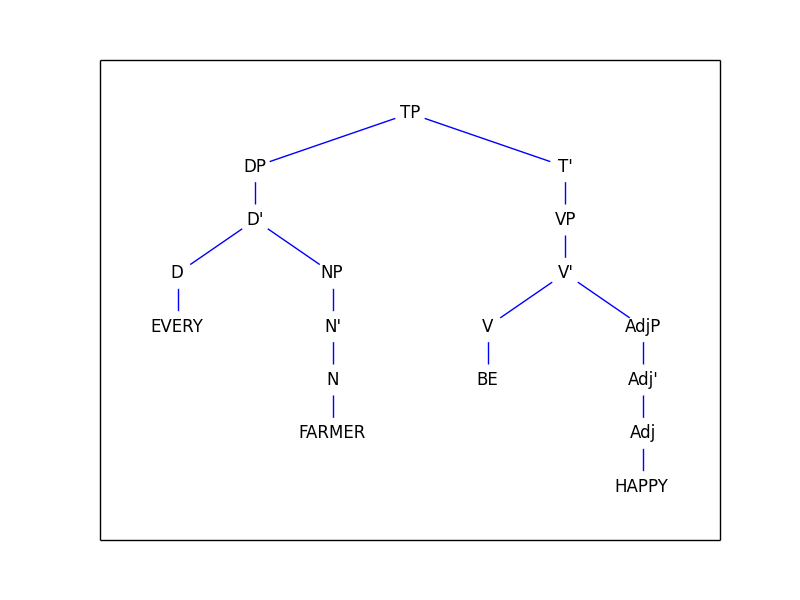
\includegraphics[scale=.7]{happy_eng_3.png}}
\caption{Morphology-bare tree, after quantifier lowering} \label{farmer_happy}
\end{figure}

\subsection{Deep structure tree to surface structure tree}

Next, we have to add morphological features to the terminal nodes.  This can be done by generating all possible morphological features for each leaf, then passing them up to the parents and checking whether they are consistent with the CFG's feature rules, continuing in this way until the entire tree has a consistent set of features.  It should be noted that some morphological ambiguities can arise in this phase.  For example, the sentence in Figure \ref{farmer_happy} could be translated as ``Every farmer is happy'' or ``All farmers are happy."  The two are logically equivalent, and if we want to be truly interlingual (i.e.\ the translation should depend only on the interlingual translation, not on the source sentence directly), then we will have to simply accept both as equally valid alternatives.  However, if we wish to allow the use of source sentence features, we can choose the one that matches the source sentence in number.  (Of course, in Japanese, there is no grammatical number, so again we are forced to be ambivalent).  Allowing source sentence features to factor into the morphological enrichment may also improve the efficiency of the process, since it allows for top-down feature checking in addition to bottom-up.

\subsection{Surface structure tree to output sentence}

Finally we have reached the end of our long translation journey.  The last step is completely trivial, as we just have to read off the leaves in left-to-right order to recover the target sentence.

Again, it is important to keep in mind that the output is really a generator that is actually a combinatorial product of several generators.  This may mean a large number of target sentences will be produced.  However, it may very well turn out that some of the trees with different structures will actually result in the same target sentence once it is read off of the tree.  We have not yet explored ways to prune the space of possible translations, but we believe that this is possible.

\section{HOLI QUAIL: Advantages and Challenges}

HOLI QUAIL is an interlingual machine translation system that can handle the subtle complexities of quantificational expressions.  This is something that pure statistical MT (including syntax-based models) cannot do.  It uses logical equivalence as the criterion for translation equivalence, which is a very well-defined notion.  The ability to convert natural language sentences into logic also allows HOLI QUAIL to act as a machine intelligence engine.  That is, it can be provided with a ``model of the world'' that a user could hypothetically query.  Logical reasoning could be conducted via automated theorem-proving and model-building tools, which have improved significantly in the past couple decades.

Another strength is that it can preserve meaning across syntactically disparate languages.  Take, for instance, the sentence ``John wa Mary ga suki desu" (``John likes Mary") into English.  The syntactic structure is actually very different between the two languages, since in Japanese, the word \textit{suki} is an adjective or noun roughly meaning ``preferred'' or ``favorite". ``Mary'' is actually the subject of the sentence, and ``John'' is the topic.  This is very dissimilar to English, where ``John'' is the subject, and ``Mary'' is the object of a transitive verb ``likes'' (see Figure \ref{eng_jap}).  Nonetheless, HOLI QUAIL has no trouble translating the Japanese sentence into English, while even the reputable Google Translate emits the egregious ``John Mary is like."

\begin{figure} [ht]
\centerline{
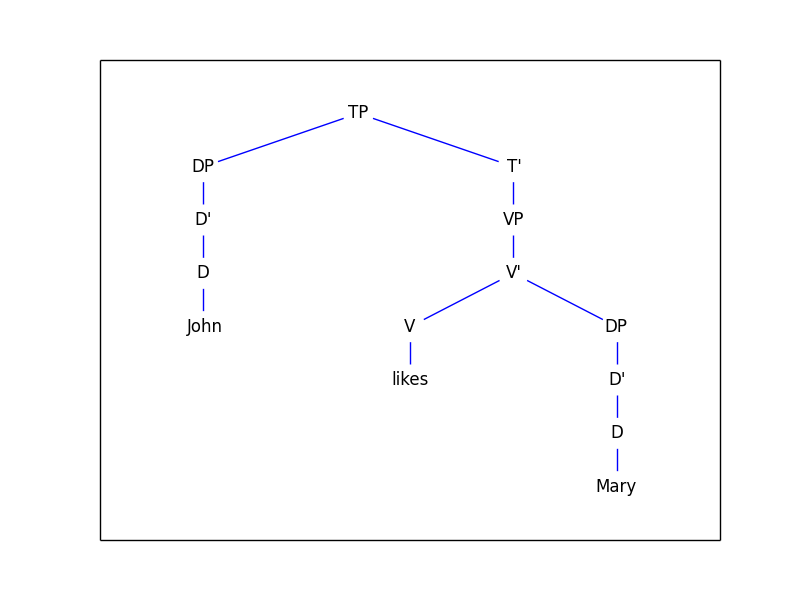
\includegraphics[scale=.5]{likes_eng_1.png}
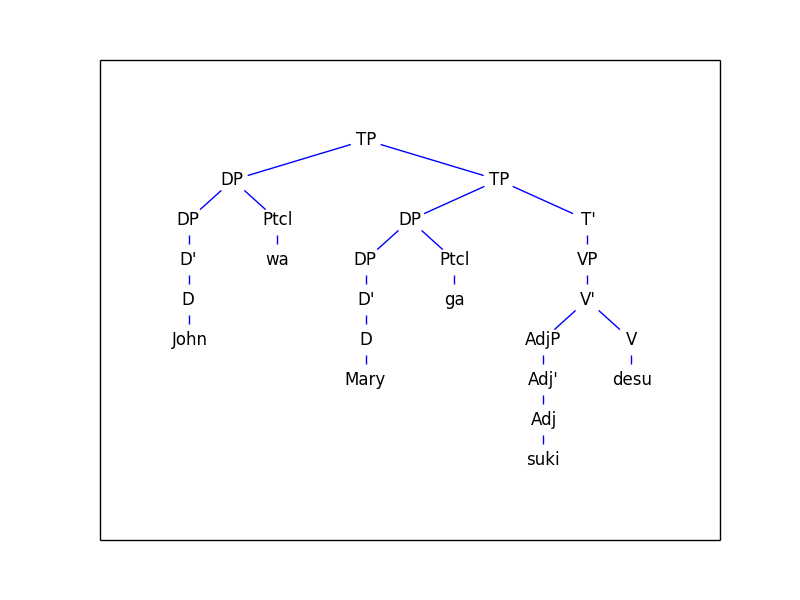
\includegraphics[scale=.5]{likes_jap_1.png}}
\caption{Different syntactic structures of English and Japanese sentence} \label{eng_jap}
\end{figure}

Here is a tidy to-do list for expanding HOLI QUAIL to handle a larger subset of natural language: 
\begin{itemize}
\item Allow for embedded clauses (``complementizer phrases''), which open up door to relative clauses and statements of belief, knowledge, etc.
\item Add possessives, prepositional phrases, adverbs, conjunctions, etc.
\item Handle anaphora (coreferential personal pronouns, reflexive pronouns, ``one'' and ``do-so'' replacement).
\item Incorporate a wider range of syntactic movement operations, and allow for parsing that inserts traces when necessary.  Doing so will likely increase the complexity of the parsing a great deal, so probabilistic parsing may be necessary.
\end{itemize}

And the following is a list of much more difficult things to explore:
\begin{itemize}
\item Incorporate tense and aspect into the semantic representation (these require temporal logic, involving quantification over times).
\item Include modals and conditionals (these require modal logic, involving quantification over ``possible worlds'').
\item Handle noncompositionality (cases where terms don't semantically combine in the ways we have described.  For instance, ``alleged murderer'' are not always murderers, so the rule of predicate modification does not apply).
\item Reason across sentence boundaries.
\item Introduce pragmatics, i.e.\ inferring the referents of anaphors from context, grasping implications of sentences, deciding the level of formality to use.
\end{itemize}

One of the biggest limitations of HOLI QUAIL is that it does not make use of probability or statistics at all.  Doing so would likely aid the performance of just about every one of its translation steps, from lexical disambiguation to morphological feature assignment.  Exhausting over possibilities in some kind of likelihood order would help to prune the large search space (very similarly to tree pruning in phrase-based decoding systems).  And although we initially emphasized that human experts would design the lexicon, their job could be assisted by an initial statistical sweep of corpus data to generate a presumptive lexicon that may only need slight tweaking by humans.  Finally, it may be beneficial to interface with a conceptual database such as WordNet so that the condition of logical equivalence could be weakened to something like ``strong semantic similarity," where this is some measurable quantity in a graph-theoretic sense.

As a fledgling effort to revive interlingua-based MT with a modern view of both linguistics and computation, HOLI QUAIL is successful in demonstrating the effectiveness of formal methods in translation.  Integrating such methods into the already successful domain of statistical MT may be the key to bringing machine translation to the next level.

\begin{thebibliography}{1}

\bibitem{nltk} Bird, Steven, Edward Loper and Ewan Klein, {\em Natural Language Processing with Python}. O'Reilly Media Inc., 2009.

\bibitem{bosBlackburn} Blackburn, Patrick, and Johan Bos.  ``Computational Semantics.''  {\em Theoria}, 18(1), pages 365-387, 2003.

\bibitem {kant} Carbonell, J., T. Mitamura and E. Nyberg. {\em The KANT Perspective: A Critique of Pure Transfer (and Pure Interlingua, Pure Statistics...)}. Carnegie Mellon University Institute for Software Research, 1999.

\bibitem {carnie} Carnie, Andrew. {\em Syntax: A Generative Introduction}. Blackwell, 2007.

\bibitem {unitran} Dorr, Bonnie. {\em UNITRAN: An Interlingual Approach}. From {\em AAAI-87 Proceedings}, M.I.T.\ Artificial Intelligence Laboratory, 1987.

\bibitem {heim} Heim, Irene, and Angelika Kratzer.  {\em Semantics in Generative Grammar}.  Blackwell, 1998.

\bibitem {mill} Mill, Bill.  {\em Drawing Presentable Trees}.  http://billmill.org/pymag-trees/

\end{thebibliography}

\end{document}  
